\nonumchapter{绪言}

在日常生活和生产劳动里,我们常常会碰到各种各样的东西,脑子里常常会出现许许多多的问题。
例如,火是什么现象?水是什么物质?水为什么能灭火?
铁是什么物质?铁和木头为什么会不一样?铁器为什么会生锈?
为什么涂上油就能防止生锈?铁是怎样炼出来的?
植物吸收空气、水等后,怎样会变成蛋白质、油脂、纤维素、糖等。
这些问题有的看起来好象很简单,但是,要正确地回答这一类问题,我们必须学习另一门自然科学——化学。

化学是研究什么的呢?在一个千变万化的物质世界里,各种各样的物质到底是由哪些成分组成的呢?
它们的内部结构是怎样的呢?它们又具有什么样的性质和变化规律呢?
以及我们可以用什么方法来合成自然界里没有的新物质、新材料呢?这些都是化学所要研究的课题。
化学是一门基础自然科学,它研究物质的组成、结构、性质、变化以及合成等。

现在我们先谈谈物质的变化和性质。

物质在不停地变化着。水冷到 $0$ ℃ 时会结成冰,水蒸发时吸收热量变成水蒸气,
但表面上不一样的液态的水、固态的冰和气态的水蒸气都是同一种物质。
固态铁受热到 $1535$ ℃ 时熔化变成液态铁,继续受热到 $2750$ ℃ 时沸腾,变成气态铁,
但表面不一样的固态铁、液态铁和气态铁也都是同一种物质。
水由液态变为固态或气态,铁由固态变为液态或气态,都只是物质的状态发生了变化,
并没有生成其它物质。我们把这种\zhongdian{没有生成其它物质的变化叫做物理变化}。
我们日常看到的象汽油的挥发、木材制成桌椅、铁铸成锅、蜡受热熔化等都是物理变化。
物理变化是物质运动的一种形式。

木柴燃烧后变成了二氧化碳、水蒸气和灰烬,这些都是不同于木柴的其它物质。
铁在潮湿的空气里生锈,铁锈是不同于铁的物质。
我们还可以把自然界和日常生活里某些物质发生变化后生成其它物质的某些现象,通过实验表现出来。

\begingroup
\renewcommand{\theshiyan}{\arabic{shiyan}}
\renewcommand{\thefigure}{\arabic{figure}\;}

\begin{shiyan}
用坩埚钳夹住镁带,点燃(图 \ref{fig:xy-1}),仔细地观察发生的现象。
\end{shiyan}

\begin{figure}[htbp]
    \centering
    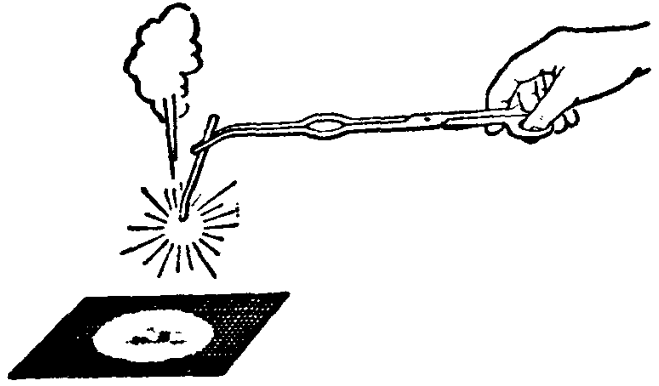
\includegraphics[width=0.7\textwidth]{../pic/czhx1-xy-1}
    \caption{镁带的燃烧}\label{fig:xy-1}
\end{figure}

镁带燃烧时发出耀眼的强光,放出大量的热,生成一种不同于镁的白色固态物质 —— 氧化镁。
镁带燃烧的变化,可表示如下:
\begin{fangchengshi}
    \ce{\text{镁} + \text{氧气} ->[\text{点燃}] \text{氧化镁}}
\end{fangchengshi}

\begin{shiyan}
把少量碳酸氢铵(一种化学肥料)放进干燥的试管里,加热, 仔细地观察发生的现象。
把火移去。用装有玻璃弯管的橡皮塞塞好试管,把玻璃弯管伸入烧杯内的澄清的石灰水里(图 \ref{fig:xy-2})。
再加热,直到碳酸氢铵完全消失。再仔细地观察发生的现象。
\end{shiyan}

\begin{figure}[htbp]
    \centering
    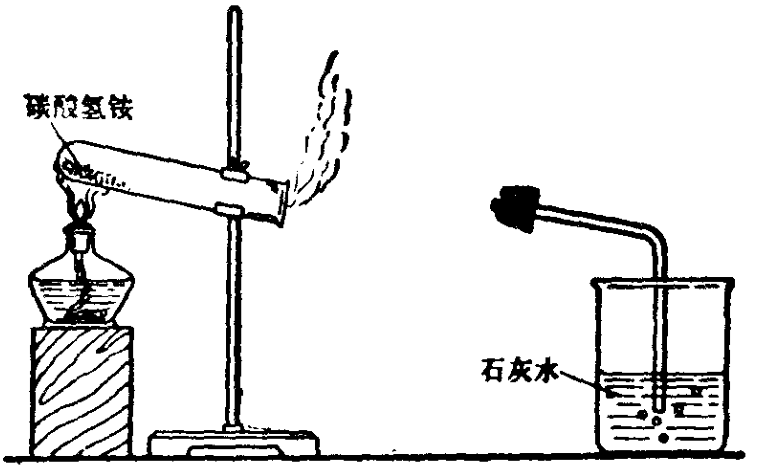
\includegraphics[width=0.7\textwidth]{../pic/czhx1-xy-2}
    \caption{加热碳酸氢铵}\label{fig:xy-2}
\end{figure}

给碳酸氢铵加热时,开始嗅到的是一股有刺激性的气味,这是氨的气味,同时试管壁上出现了水珠。
从玻璃弯管放出的气体使澄清的石灰水逐渐变浑浊,使澄清的石灰水变浑浊是二氧化碳的特性。
从这些现象知道,碳酸氢铵受热分解产生氨气、水和二氧化碳三种其它的物质,并且可以表示如下:
\begin{fangchengshi}
    \ce{\text{碳酸氢铵} ->[\text{加热}] \text{氨气} + \text{水} + \text{二氧化碳}}
\end{fangchengshi}

\endgroup

分析上面两个实验,可以知道它们有一个共同的特征,就是
\zhongdian{变化时都生成了其它的物质,这种变化叫做化学变化,}又叫做\zhongdian{化学反应}。
上面提到的木柴的燃烧和铁在潮湿的空气里生锈都是化学变化。
其他象铁矿石炼成铁、炸药的爆炸等也都是化学变化。化学变化是物质运动的另一种形式。

化学变化的特征是生成了新的物质。在化学变化的过程中,常伴随着发生一些现象,
如放热、发光、变色、放出气体、生成沉淀等等。这些现象常常可以帮助我们判断有没有化学变化发生。

化学变化和物理变化常常同时发。在化学变化过程里一定同时发生物理变化。
例如,点燃蜡烛时,蜡受热熔化是物理变化,同时蜡又燃烧生成水和二氧化碳,却是化学变化。
但在物理变化的过程里不一定发生化学变化。

\zhongdian{物质在化学变化中表现出来的性质叫做化学性质。}
例如,镁能在空气中燃烧,生成氧化镁,碳酸氢铵受热会生成氨、水、二氧化碳等。
\zhongdian{物质不需要发生化学变化就表现出来的性质,如颜色、状态、气味、熔点、沸点、硬度、密度等,叫做物理性质。}

我们学习化学,掌握化学变化规律,既可提炼出自然界原来就存在的物质,
也可以制造出自然界原来并不存在的物质,为提高人民的物质生活水平服务。
用空气、水和石油、天然气或煤可以制造化肥和炸药;
用水、食盐可以生产烧碱、氯气、盐酸;
用石油或天然气可以制出五光十色的塑料、巧夺天工的合成纤维、
品质优良的合成胶、去污除垢的合成洗涤剂、鲜艳夺目的染料、除疾去病的药品。
研究生命现象,研制新型材料,制造宇宙飞船,探究星际物质的组成以及探索新的能源,都要用到化学知识。
另一方面,掌握化学变化规律,还可以控制对人类利益有害的变化,为消除大气和水的污染、
环境的破坏以及处理原子废物等威胁人类生存的祸患而奋斗。

在我们的日常生活中,象怎样防火、灭火,怎样防止铁生锈,怎样使用发酵粉,
怎样净化水和软化硬水等,都要用到化学知识。

我国是世界文明发达最早的国家之一,对人类作出过巨大的贡献。
我国有些化学工艺发明较早,象造纸、制火药、烧瓷器都是世界闻名的。
我国劳动人民早在商代就会制造青铜器,春秋晚期就会冶铁,战国晚期就会炼钢。
只是到了近代,由于封建制度的日益腐败,外国的侵略,统治阶级的黑暗反动,
我国的科学技术发展停滞了,大大落后了。解放前我国的工业生产处于极端落后的状态。
大多数化学工厂只拿进口的材料和半成品进行简单的加工,甚至连煤油、烧碱、火柴等都要从外国进口。
解放后,我国的石油、化学等工业起了巨大的变化,化学科学研究也不断取得了新的成就。
拿石油工业来说,我国石油工人和科学技术人员已经高速度、高质最地开发并建设了世界上较大油田——大庆油田,
还陆续建成了胜利、大港等油田,结束了中国用“洋油”的历史。
我国的化学工业已发展成为一个具有一定规模、行业基本齐全的工业部门。
以石油为原料的合成树脂与塑料、合成纤维、合成橡胶三大合成材料工业,也迅速地发展起来。
我国在世界上首先人工合成了蛋白质和核糖核酸\footnotemark,对探索生命的奥秘有着重要意义。
我国原子弹、氢弹、导弹的试验成功,人造地球卫星的发射和准确回收,
集中标志着我国科学技木包括化学科学技术在内达到新的水平。
\footnotetext{蛋白质指的是结晶牛胰岛素。核糖核酸指的是酵母丙氨酸转移核糖核酸。}

化学与建设我们伟大的社会主义的现代化强国有着密切的关系。
例如,现代农业需要大量化肥,需要高效肥料、复合肥料、微量元素肥料、
高效低毒低残留农药、除草剂、植物生长刺激素、人工降雨化学药剂等等;
现代工业需要耐高温、耐腐蚀、不燃烧的高分子材料,具有最佳性能的酶催化剂等等;
现代科学技术和现代国防特殊需要的化工材料和产品象原子反应堆用的重水,
导弹、飞机用的轻质非金属材料,火箭的推进剂,电子工业用的高纯物质和特纯试剂等等。
这些材料和产品的生产都要直接用到化学知识。

同学们!现在你们幸福地在校里学习,将来,你们要投身于社会主义建设的战斗岗位,
到那时,祖国社会主义现代化的建设事业将迈出更大的步伐,
展现在你们面前的是多么广阔美好的前景,交给你们的担子是多么的重大。
希望你们树雄心,立壮志,为社会主义祖国的四个现代化学好化学。
在学习化学中要牢固地、系统地掌握化学基础知识和基本技能;
坚持理论联系实际的原则,了解这些知识和技能在工农业生产和科学技术上的应用;
逐步培养辩证唯物主义观点,为攀登科学技术高峰打好坚实的基础。
化学是一门以实验为基础的科学,要认认真真地做好化学实验。
在化学实验中,要集中注意力,运用各种感官,细致耐心地进行观察,
详细、准确、如实地做好记录,并根据实验得出结论,找寻规律。
在掌握础知识和基本技能的过程中,要逐步提高自己的观察能力、思维能力、自学能力和独立操作能力等。
希望你们立志成为有社会主义觉悟的有文化的劳动者,用火红的青春去谱写伟大的社会主义祖国四个现代化的壮丽诗篇。


\begin{xiti}

\xiaoti{物理变化和化学变化有什么区别?试举几个日常生活中看到的现象来说明。}

\xiaoti{下列现象哪些是物理变化,哪些是化学变化? 为什么?}
\begin{xiaoxiaotis}

    \xxt{钢铁生锈,}

    \xxt{澄清的石灰水中通入二氧化碳后变浑浊,}

    \xxt{冰融化成水,}

    \xxt{食物腐烂,}

    \xxt{火药爆炸,}

    \xxt{煤的燃烧,}

    \xxt{钢锭轧成钢条,}

    \xxt{矿石粉碎。}

\end{xiaoxiaotis}

\xiaoti{举例说明化学跟把我国建设成为伟大的社会主义的现代化强国有什么关系。}

\end{xiti}

